%%%%%%%%%%%%%%%%%%%%%%%%%%%%%
% Standard header for working papers
%
% WPHeader.tex
%
%%%%%%%%%%%%%%%%%%%%%%%%%%%%%

\documentclass[11pt]{article}

%%%%%%%%%%%%%%%%%%%%
%% Include general header where common packages are defined
%%%%%%%%%%%%%%%%%%%%



%%%%%%%%%%%%%%%%%%%%%%%%%%
%% Packages
%%%%%%%%%%%%%%%%%%%%%%%%%%


% general packages without options
\usepackage{amsmath,amssymb,bbm}

% graphics
\usepackage{graphicx}

% text formatting
\usepackage[document]{ragged2e}
\usepackage{pagecolor,color}




\usepackage[utf8]{inputenc}
\usepackage[T1]{fontenc}
%\usepackage[francais]{babel}



% for framed figures or texts
\usepackage{mdframed}



%%%%%%%%%%%%%%%%%%%%
%% Idem general commands
%%%%%%%%%%%%%%%%%%%%
%% Commands

\newcommand{\noun}[1]{\textsc{#1}}


%% Math

% Operators
\DeclareMathOperator{\Cov}{Cov}
\DeclareMathOperator{\Var}{Var}
\DeclareMathOperator{\E}{\mathbb{E}}
\DeclareMathOperator{\Proba}{\mathbb{P}}

\newcommand{\Covb}[2]{\ensuremath{\Cov\!\left[#1,#2\right]}}
\newcommand{\Eb}[1]{\ensuremath{\E\!\left[#1\right]}}
\newcommand{\Pb}[1]{\ensuremath{\Proba\!\left[#1\right]}}
\newcommand{\Varb}[1]{\ensuremath{\Var\!\left[#1\right]}}

% norm
\newcommand{\norm}[1]{\| #1 \|}


%% graphics

% renew graphics command for relative path providment only ?
%\renewcommand{\includegraphics[]{}}



% geometry
\usepackage[margin=2cm]{geometry}

\usepackage{float}

% layout : use fancyhdr package
\usepackage{fancyhdr}
\pagestyle{fancy}

\makeatletter

\renewcommand{\headrulewidth}{0.4pt}
\renewcommand{\footrulewidth}{0.4pt}
\fancyhead[RO,RE]{15-17/03/2017}
\fancyhead[LO,LE]{TP1}
\fancyfoot[RO,RE] {\thepage}
\fancyfoot[LO,LE] {L1 54BEG3GO - S2 2017}
\fancyfoot[CO,CE] {}


\fancypagestyle{firststyle}
{
   \fancyhf{}
   \fancyhead[RO,RE]{TP1 - 15-17/03/2017}
   \fancyhead[LO,LE]{L1 54BEG3GO - S2 2017}
}


%\renewcommand{\abstractname}{Objectifs du TD}

\renewcommand{\figurename}{\textbf{Document}}


\makeatother


%%%%%%%%%%%%%%%%%%%%%
%% Begin doc
%%%%%%%%%%%%%%%%%%%%%

\begin{document}









\title{\textbf{Statistiques et Cartographie - TP1}}

\date{}


\maketitle

\justify

\thispagestyle{firststyle}


\textit{\textbf{Consignes : }Le tableau de données et de travail \texttt{} est à télécharger sur Moodle}


\bigskip


\section*{Exercice : Perception des Risques d'Inondation}

\paragraph{Contexte (2pts)}

% blabla contexte, quanti quali etc

\textit{}




\paragraph{Données (3pts)}

% carte de loc, commentaire



\begin{figure}
\centering
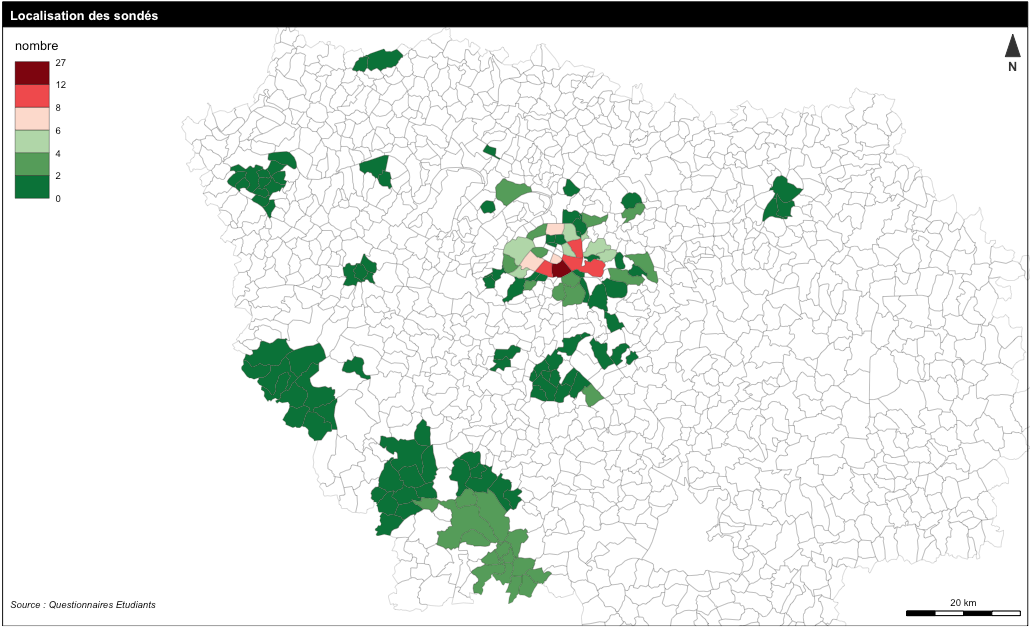
\includegraphics[width=0.8\textwidth]{maps/count2}
\caption{Nombre de réponses au sondage par communes (code postal).}
\end{figure}



\paragraph{Traitement des données (5pts)}




\paragraph{Interpretation (5pts)}



\paragraph{Point de vue cartographique (2pts)}












\bigskip
\bigskip

\strut\hfill$\star$\hspace{1.2cm}$\star$\hfill\strut\vspace{0.1cm}\\

\strut\hfill$\star$\hfill\strut\par





\section*{Exercice Facultatif}









\end{document}